\subsection{Application on AIG Datas}
\label{sec:appl-aig-datas}
\paragraph{}
In this section we will apply the previous results on quoted spreads data of the
company  AIG. The  data provided  is  a series  of  CDS quoted  spreads for  the
maturities $1,\dots,10$ between 16/08/2005 and 30/09/2010 :
\[
data\footnote{we note $S_i=S_{i,.}=(S_{i,t})_{t=t_1,\dots,t_n}$, respectively $S_t=S_{.,t}=(S_{i,t})_{i=1,\dots,10}$} = (S_{i,t})_{\ i=1,\dots,10\ (years)\ \mathrm{and}\
  t=t_1,\dots,t_n(\mathrm{quatation dates})}
\]

\subparagraph{}
The first  idea consist on studying  statistically the behavior of  spreads over
2005 - 2010. 

\begin{figure}[H]
  \centering 
  \includegraphics[width=0.8\textwidth]{dynamic_spreads}
  \caption{\it Evolution of spreads of the company AIG }
  \label{fig:5}
\end{figure}
\paragraph{}
We  can naturally  remark two  phases in  the spreads  evolution: the  first one
corresponds  to a  stagnation of  CDS  market from  0 to  600 corresponding  to
16/08/2005-03/12/2007 .  The second one remains from the surrounding of 600 to
the end  of the period  30/09/2010. This period  is exactly superimposed  to the
subprime crisis. We  can remark that the  company have reached a  hight level of
spreads. This policy  is quite  natural in  a period of  crisis, the  company had  had to
increase her spreads in presence of a hight risk of bankruptcy. \\

\paragraph{}
In almost all  quotations, spread is an increasing function  of time. Obviously,
the more  years protection recover, higher  is the risk that  the protecter most
care. But how much would the company be vulnerable to maturity ?
\paragraph{}
To do so, we computed the empirical variance of each spread quotation. 
 The following
graphic shows the spreads variances 
\[
\mathrm{Empirical\  variance\ for\  a\ quotation\  \mathit{t}} =  Var(S_{.,t}) =
\frac{1}{n}\sum_{i=1}^{10}(S_{i,t} - \overline{S_{.,t}})^2
\]
over the available maturities :

\begin{figure}[H]
  \centering
\label{fig:6}
  \includegraphics[width=0.8\textwidth]{spreads_volatility}
  \caption{\it Quoted spreads variance }
\end{figure}

In the beginning of \textit{2005-2006} we  can remark a complete indifference of
the  company against  maturity :  this reflect  that the \textit{ subprime crisis}  where
totaly unpredictable. Once  the crisis was established, the  company changed its
policy and became too vulnerable to the maturity.

\subsection{Dynamic of bounds }
\label{sec:dynamic-bounds-}

\paragraph{}
Under  \textit{arbitrage-free}  conditions, proposition  (\ref{prop:3.2})  gives
bounds for credit curves at each quotation :
\begin{figure}[H]

  \centering
  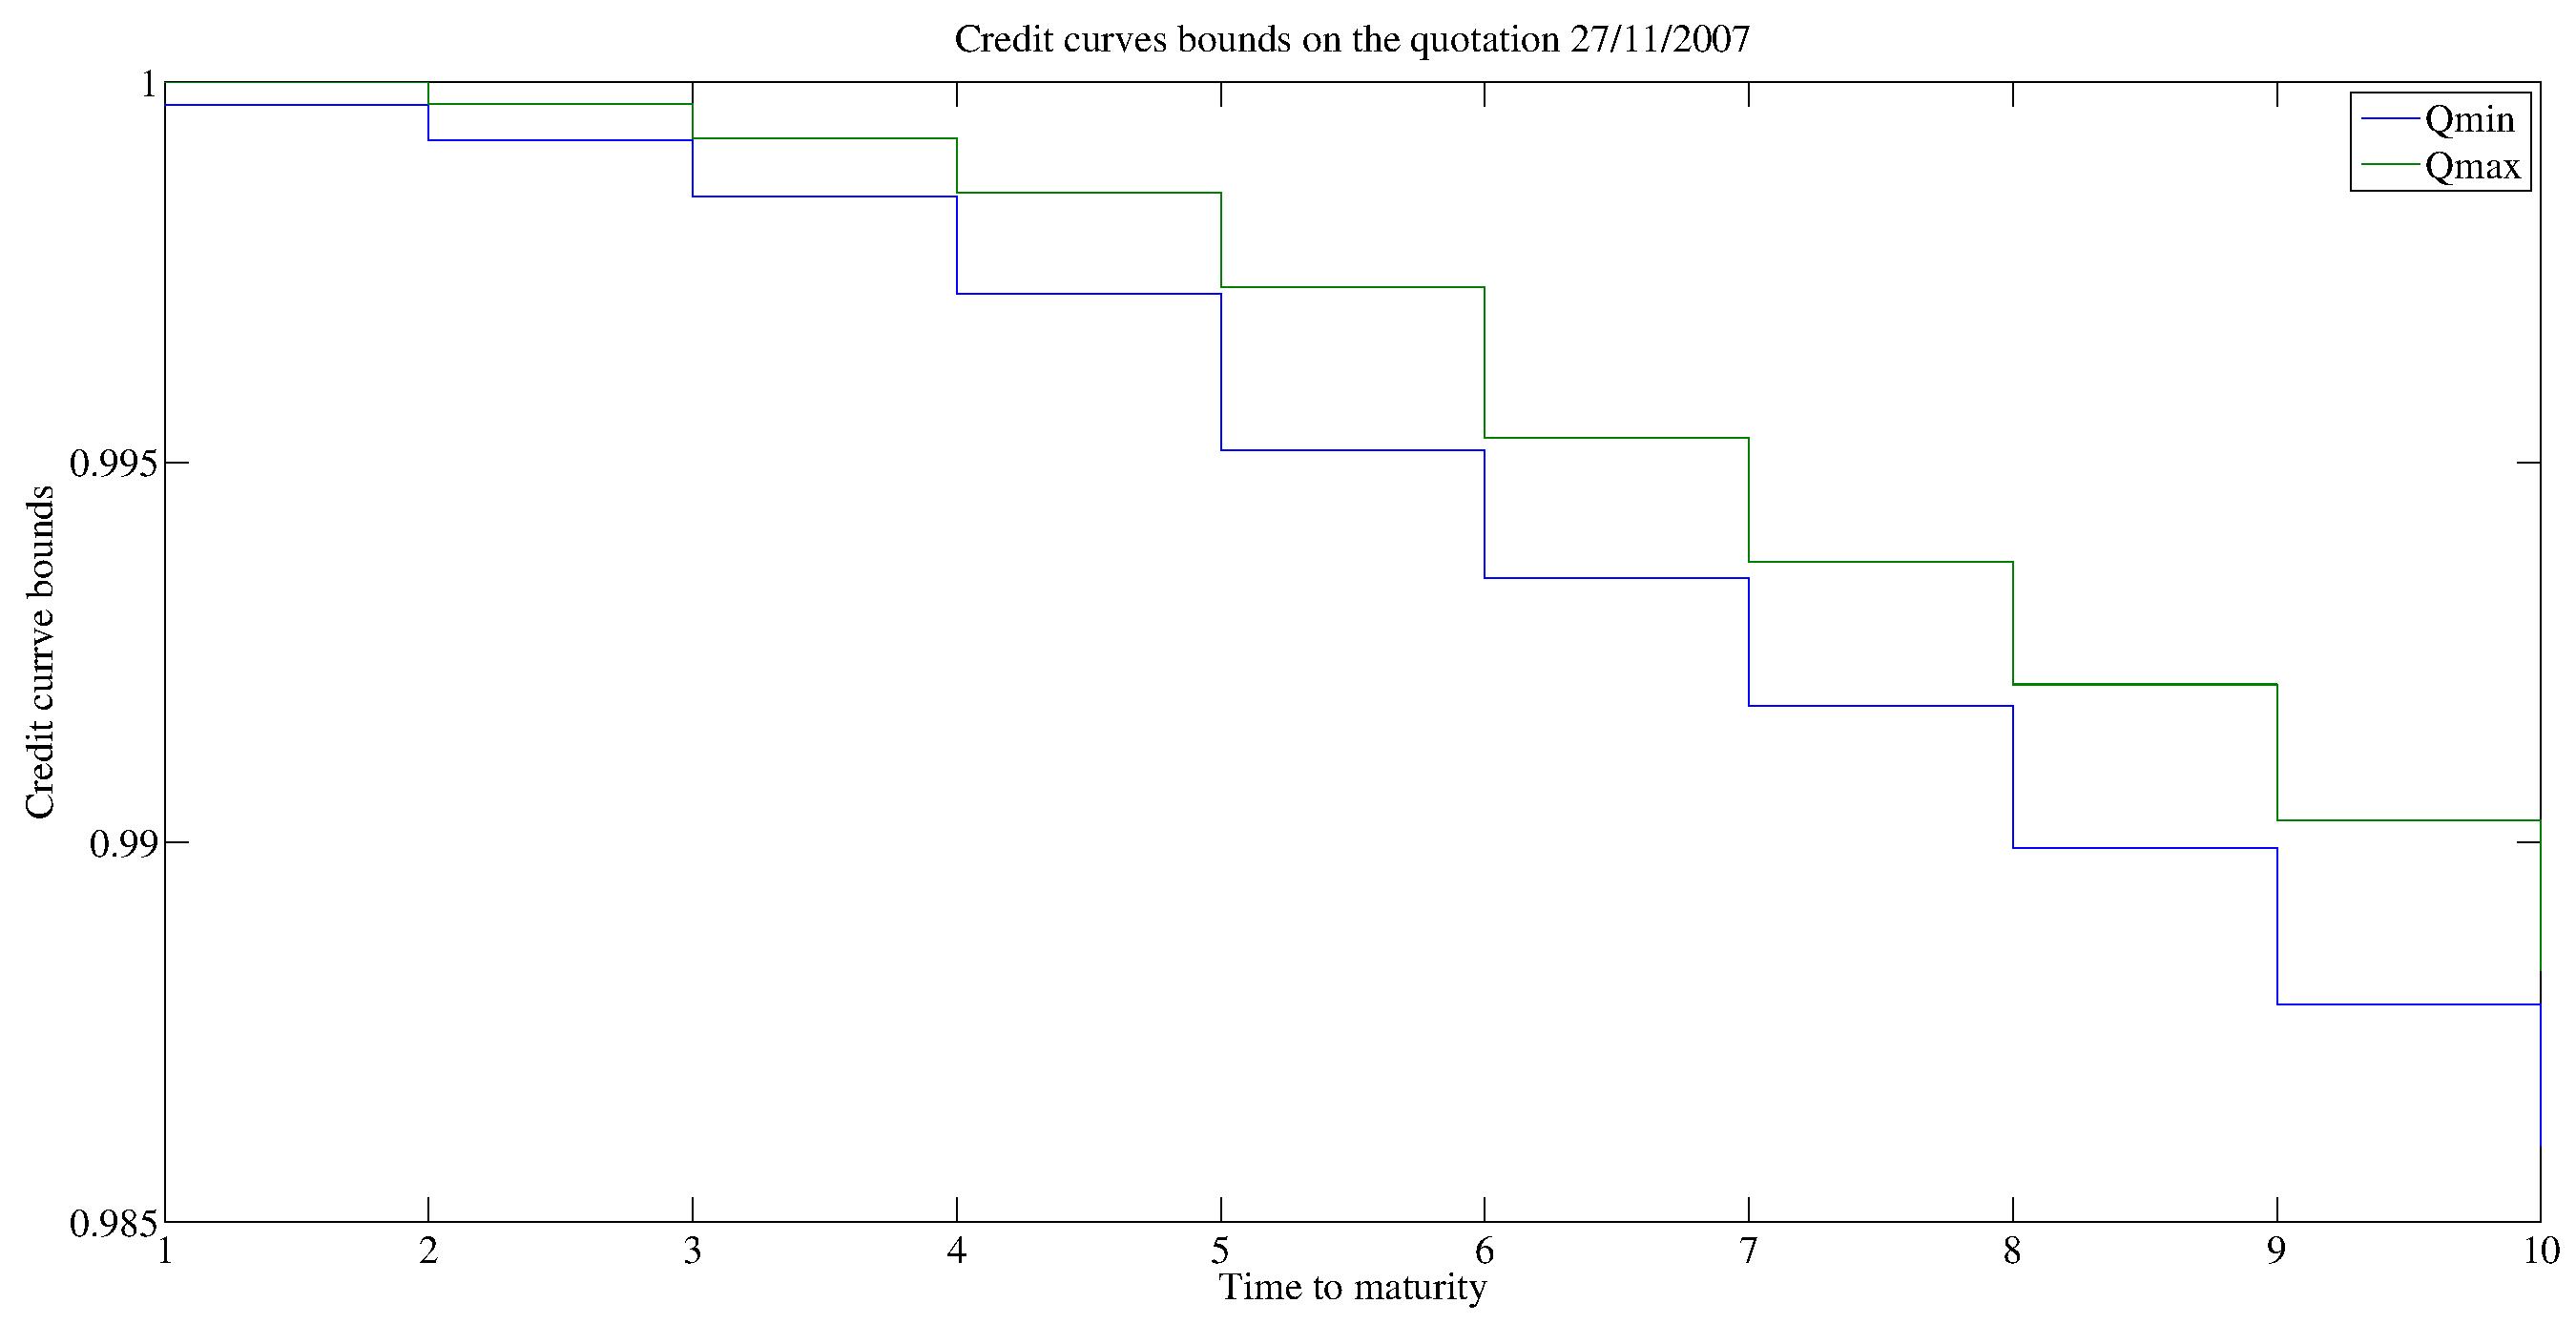
\includegraphics[width=0.8\textwidth]{cotation_27_11_2007}
  \caption{\it Credit curve among 18/08/2005 - 28/09/2007}
\label{fig7}
\end{figure}

We can  use this  proposition to
identify   either  arbitrage   free  opportunities   :  if   the  arbitrage-free
inequalities  are not  violated  that  means that  there  are  arbitrage at  the
specified quotation.  Indeed figure (\ref{fig:8}) shows an example of a quotation that
present an arbitrage opportunity :

\begin{figure}[H]
  \centering
  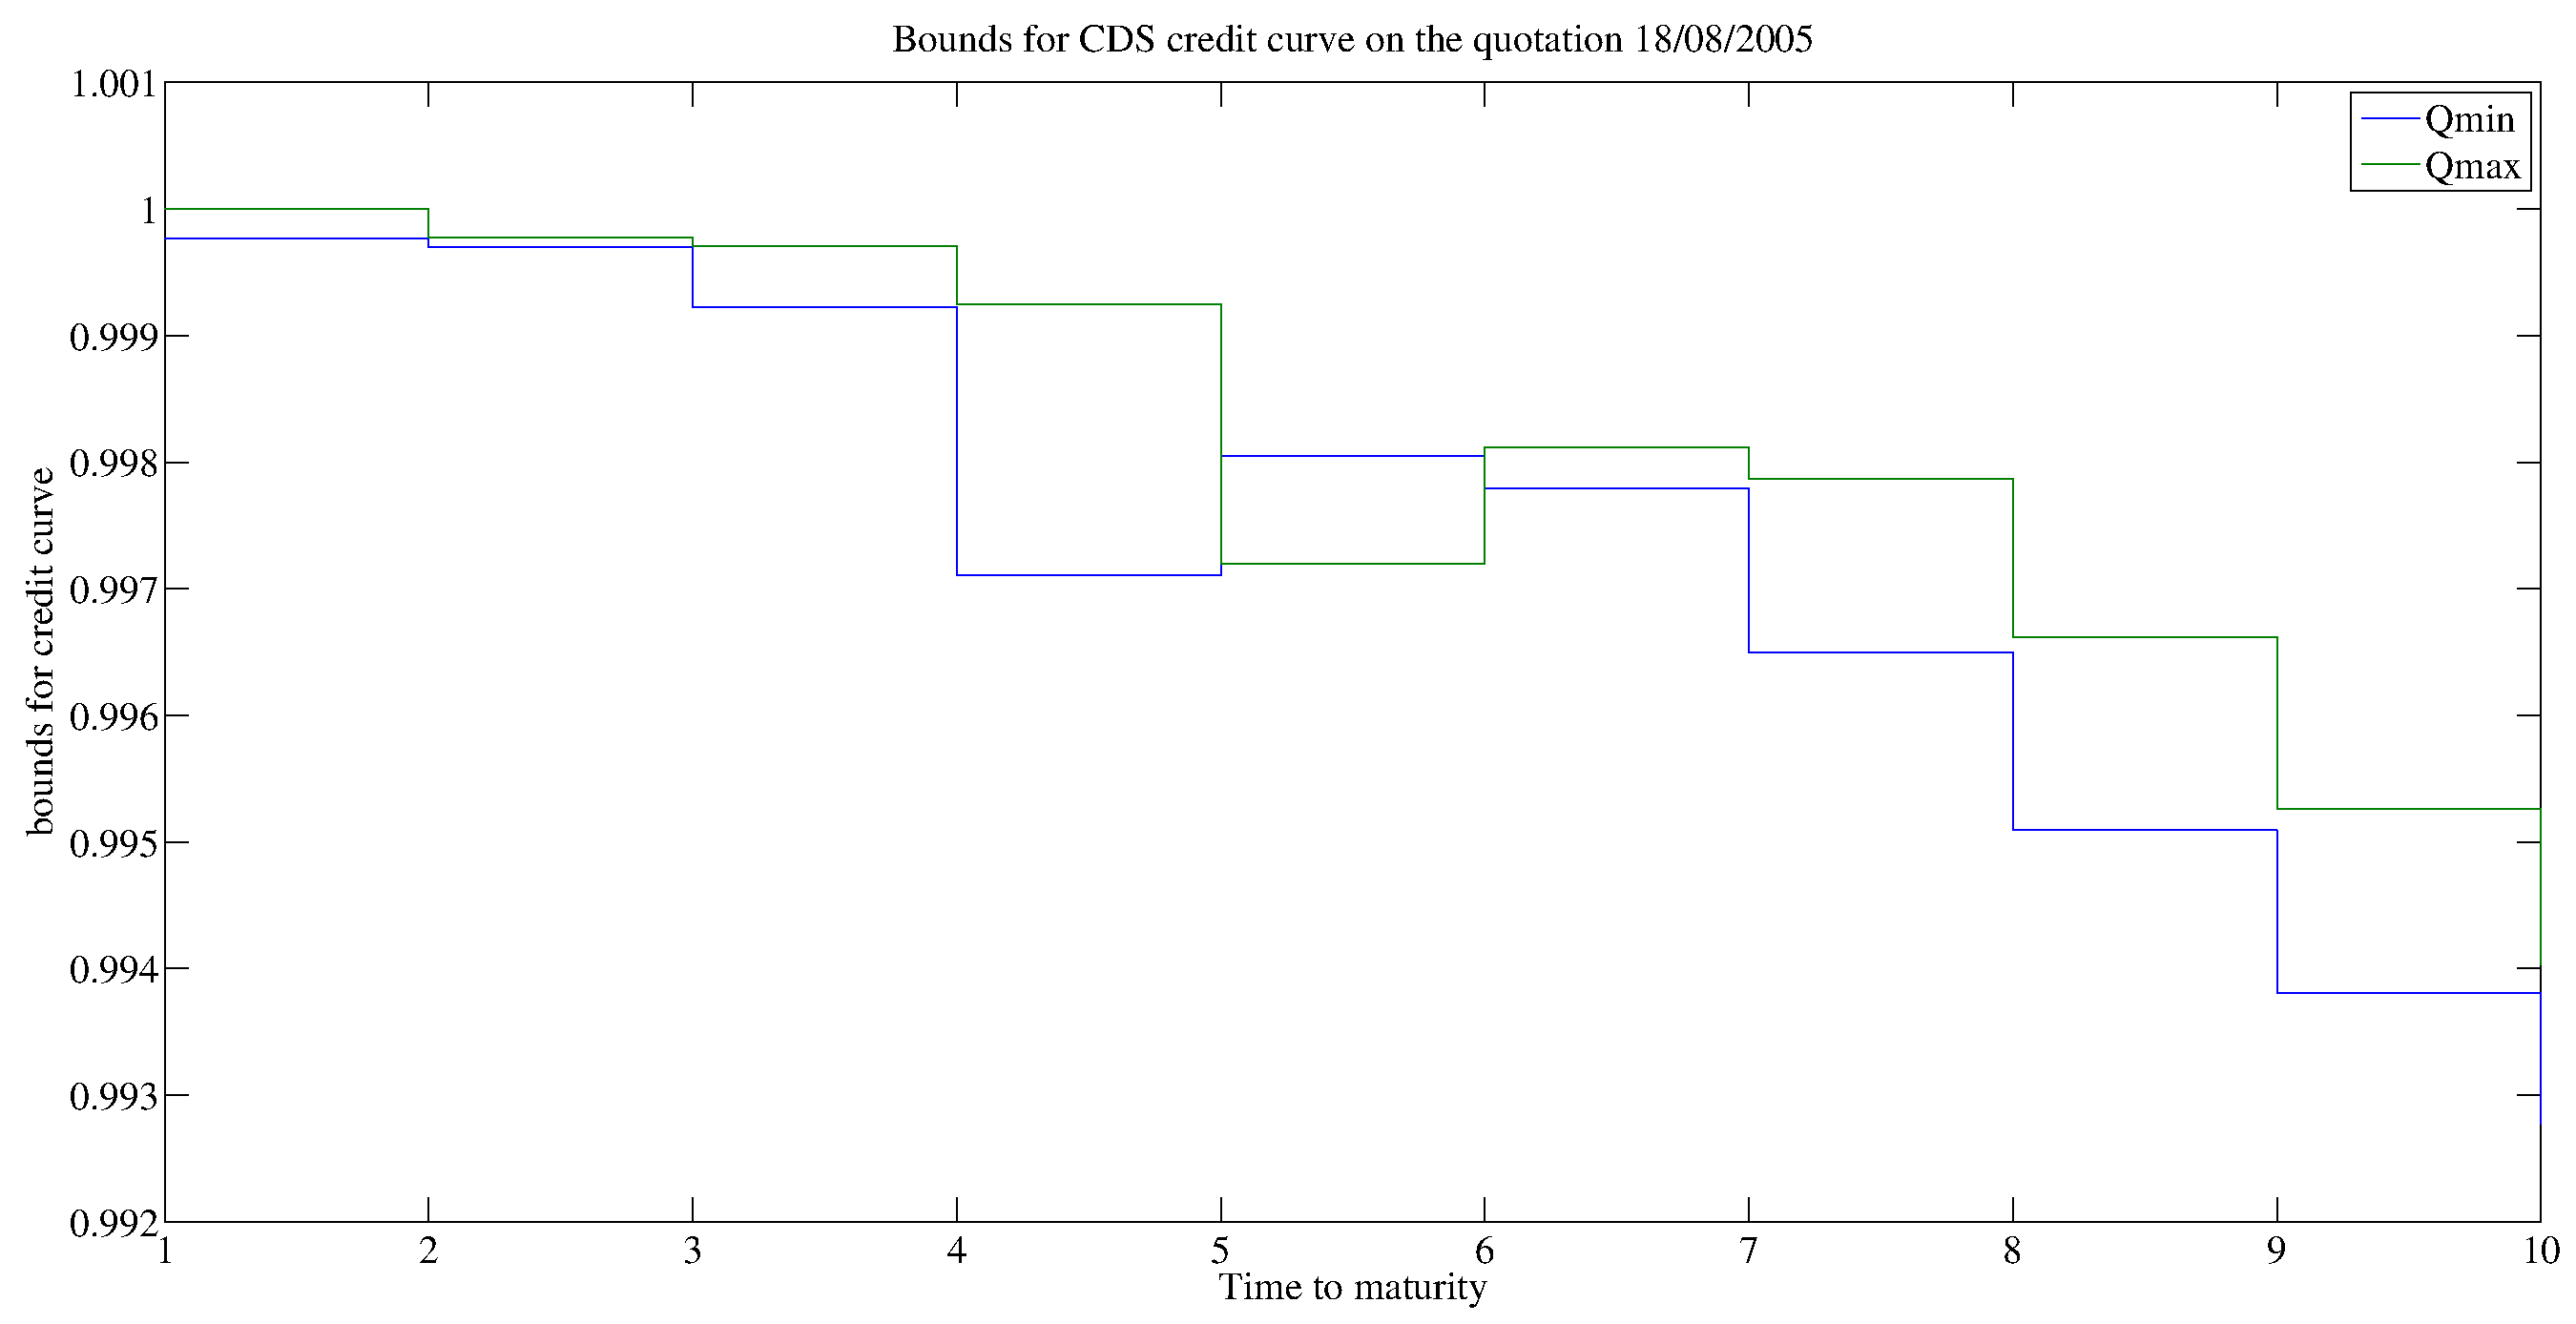
\includegraphics[width=0.8\textwidth]{cotation-18-08-2005}
  \caption{\it Market fit condition non verified}
  \label{fig:8}
\end{figure}

\paragraph{}
This   arbitrage   opportunities   remain   from  {\it   16/08/2005}   to   {\it
  28/09/2007}. After this date, the market remained obscur for arbitrage opportunities.
\paragraph{}
NB: The precision of bounds, in the meaning of the gap thickness (see \ref{gap}),
follows the same evolution as the variance.


\subsection{Bounds Dynamic}
\label{sec:bounds-effectiveness}
\paragraph{}
In order  to see how  bounds changes over spreads  quotation, we plot  the width
$Q_{max}-Q_{min}$ :
\begin{figure}[H]
  \centering
  \includegraphics[angle=-90,width=0.8\textwidth]{bounds_Dynamic_T_4}
  \caption{\it total matching with the spreads evolution for the maturity T = 4 years}
  \label{fig:10}
\end{figure}

The results  of the figure (\ref{fig:10})  remain true for all  maturities. This
result can be explained by  a positive correlation between $Q_{max}-Q_{min}$ and
$S_i$. Indeed the following figure shows a typical regression of $Q_{max}$ over $S_i$

\begin{figure}[H]
  \centering
  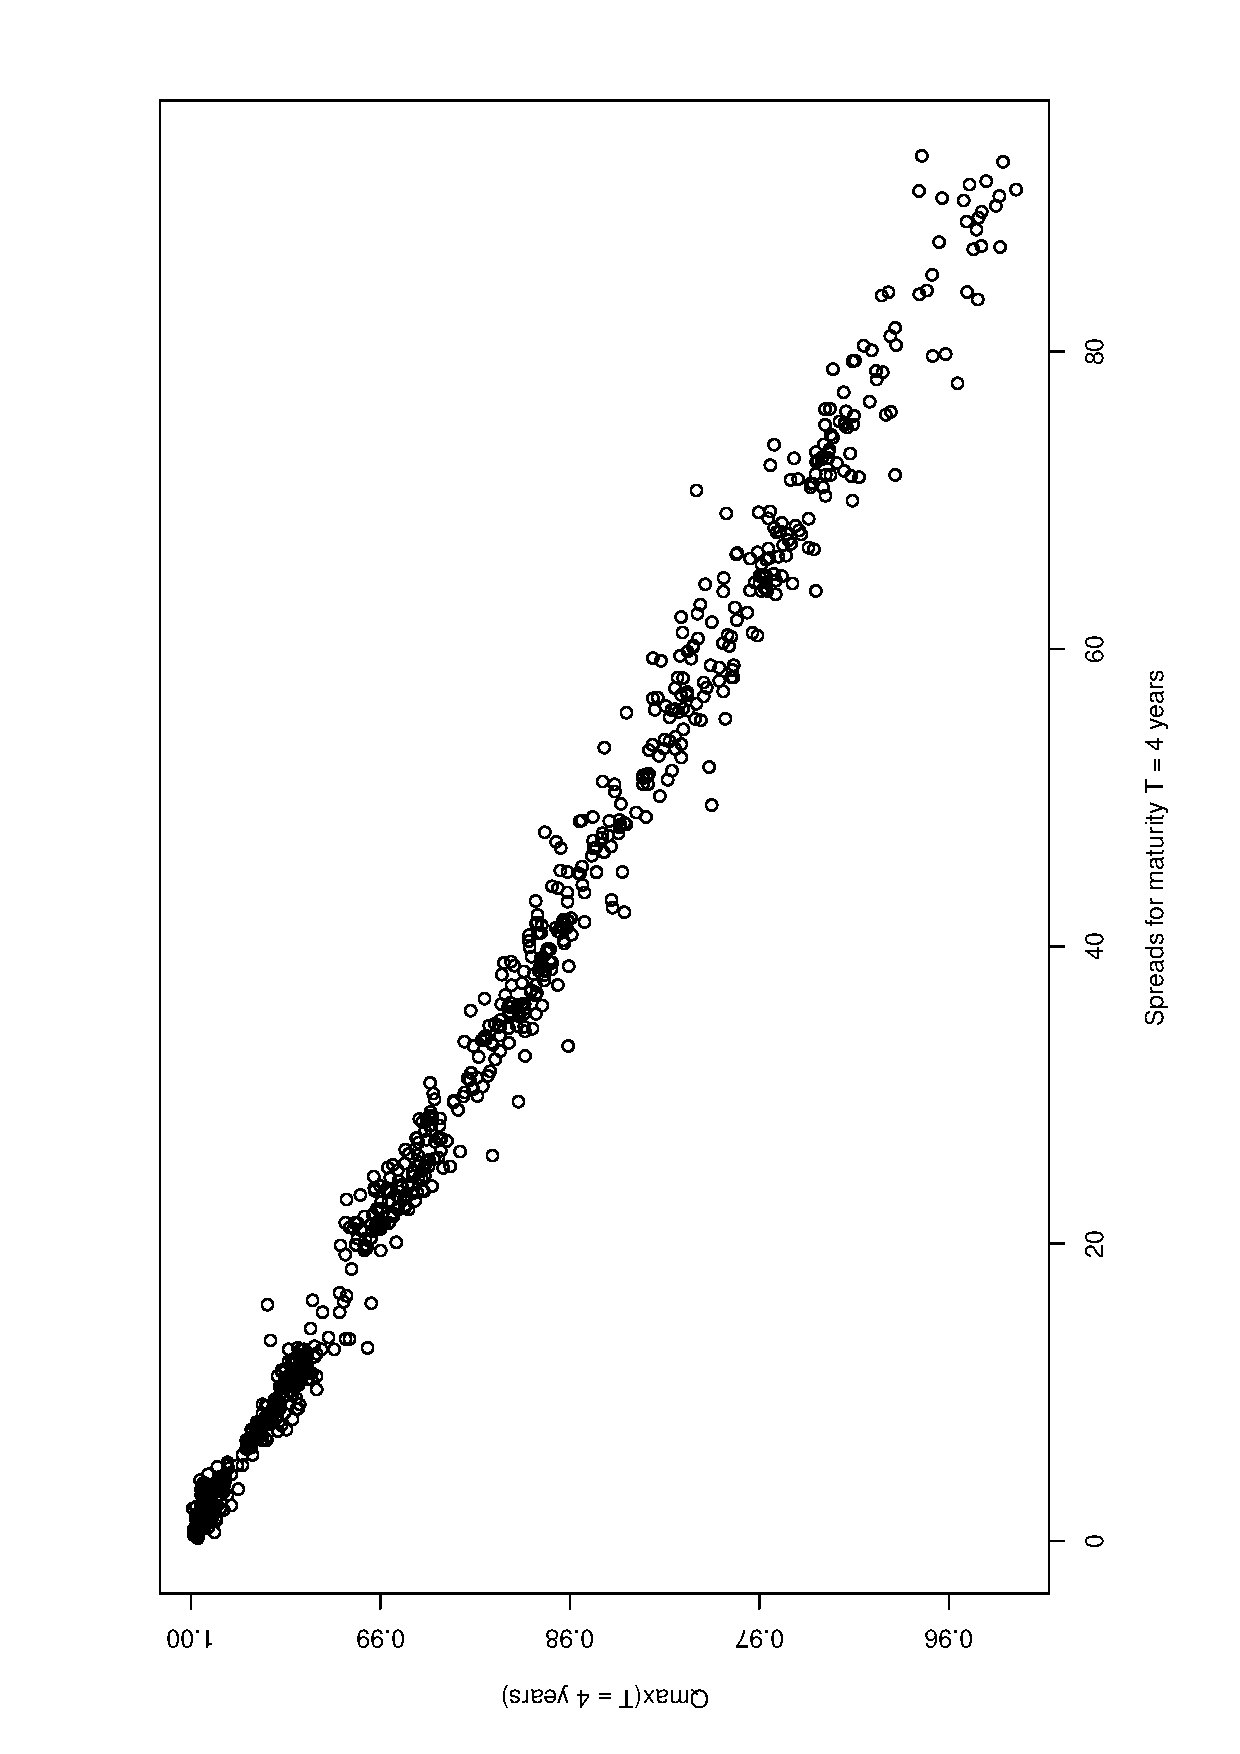
\includegraphics[angle=-90,width=0.8\textwidth]{corr_T_4}
  \caption{\it total matching with the spreads evolution for the maturity T = 4 years}
  \label{fig:11}
\end{figure}

The   same   result   remain   true   for   $Q_{min}$.   We   can   write   then
$Q_{max}-Q_{min}=\alpha_i  S_{i,.} +  \beta_i$ which  explain  that the  gap of  the
bounds $G_i  = Q_{max}-Q_{min}$ have the  same evolution as the  Spreads $S_i,.$
for each maturity $T=1,\dots,10 (years)$




\subsection{CIR model}
This  section is  the direct  continuity of  the paragraph  4 of  the article  :
A.cousin \& I.Niang section 4 \cite{OTRATS}.\\


\paragraph{}
The  construction of  admissible term-structure  is based  on CIR(Cox  Ingersoll
Ross) model 
\[
dX_t=a(b(t) - X_t)dt + \sigma \sqrt(X_t)dW_t
\]
or a Levy-driven Ornstein-Uhlenbeck process(Levy-driven OU)
\[
dX_t= a(b(t) - X_t)dt + \sigma dY_{ct}
\]
where $Y_{ct}$ is a Levy process. \\
In our furthur applications we will use the CIR model. In order to see the influence of the CIR\footnote{ we refere to the article of
}   parameters   $(a,\sigma,X_0)$.  We've   varied   the   parameter  $a$   over
$[0.01,2.00]$. We plot  then the survival probabilities, solution  of CIR model,
for a fixed $\sigma,X_0,R$ :
\begin{figure}[H]
  \centering 
    \includegraphics[angle=0,width=0.8\textwidth]{survival_a}
  \caption{survival curves for the quotation 15/06/2009 with $\sigma = 0.2 \ x_0
    = 1.6e-6$, rate $R = 40 \%$ , $P^D(t_0,t)=\exp(-R(t-t_0))$}
  \label{fig:11}
\end{figure}

the same thing for the parameter $s$ :

\begin{figure}[H]
  \centering 
    \includegraphics[angle=0,width=0.8\textwidth]{survival_s}
  \caption{survival curves for the quotation 15/06/2009 with $a = 1 \ x_0
    = 1.6e-6$, rate $R = 40 \%$ , $P^D(t_0,t)=\exp(-R(t-t_0))$}
  \label{fig:11}
\end{figure}
